
\section{Narrative workshop dataset}



\section{Museum visit dataset}

Over the course of this thesis, my research buddies and I have visited in total 10 exhibitions from 7 different museums in Oslo. From these museum visits, we have documented 22 interactive installations that forms the dataset used for analysis and similar investigations in our respective thesis's. 

\begin{figure}[H]
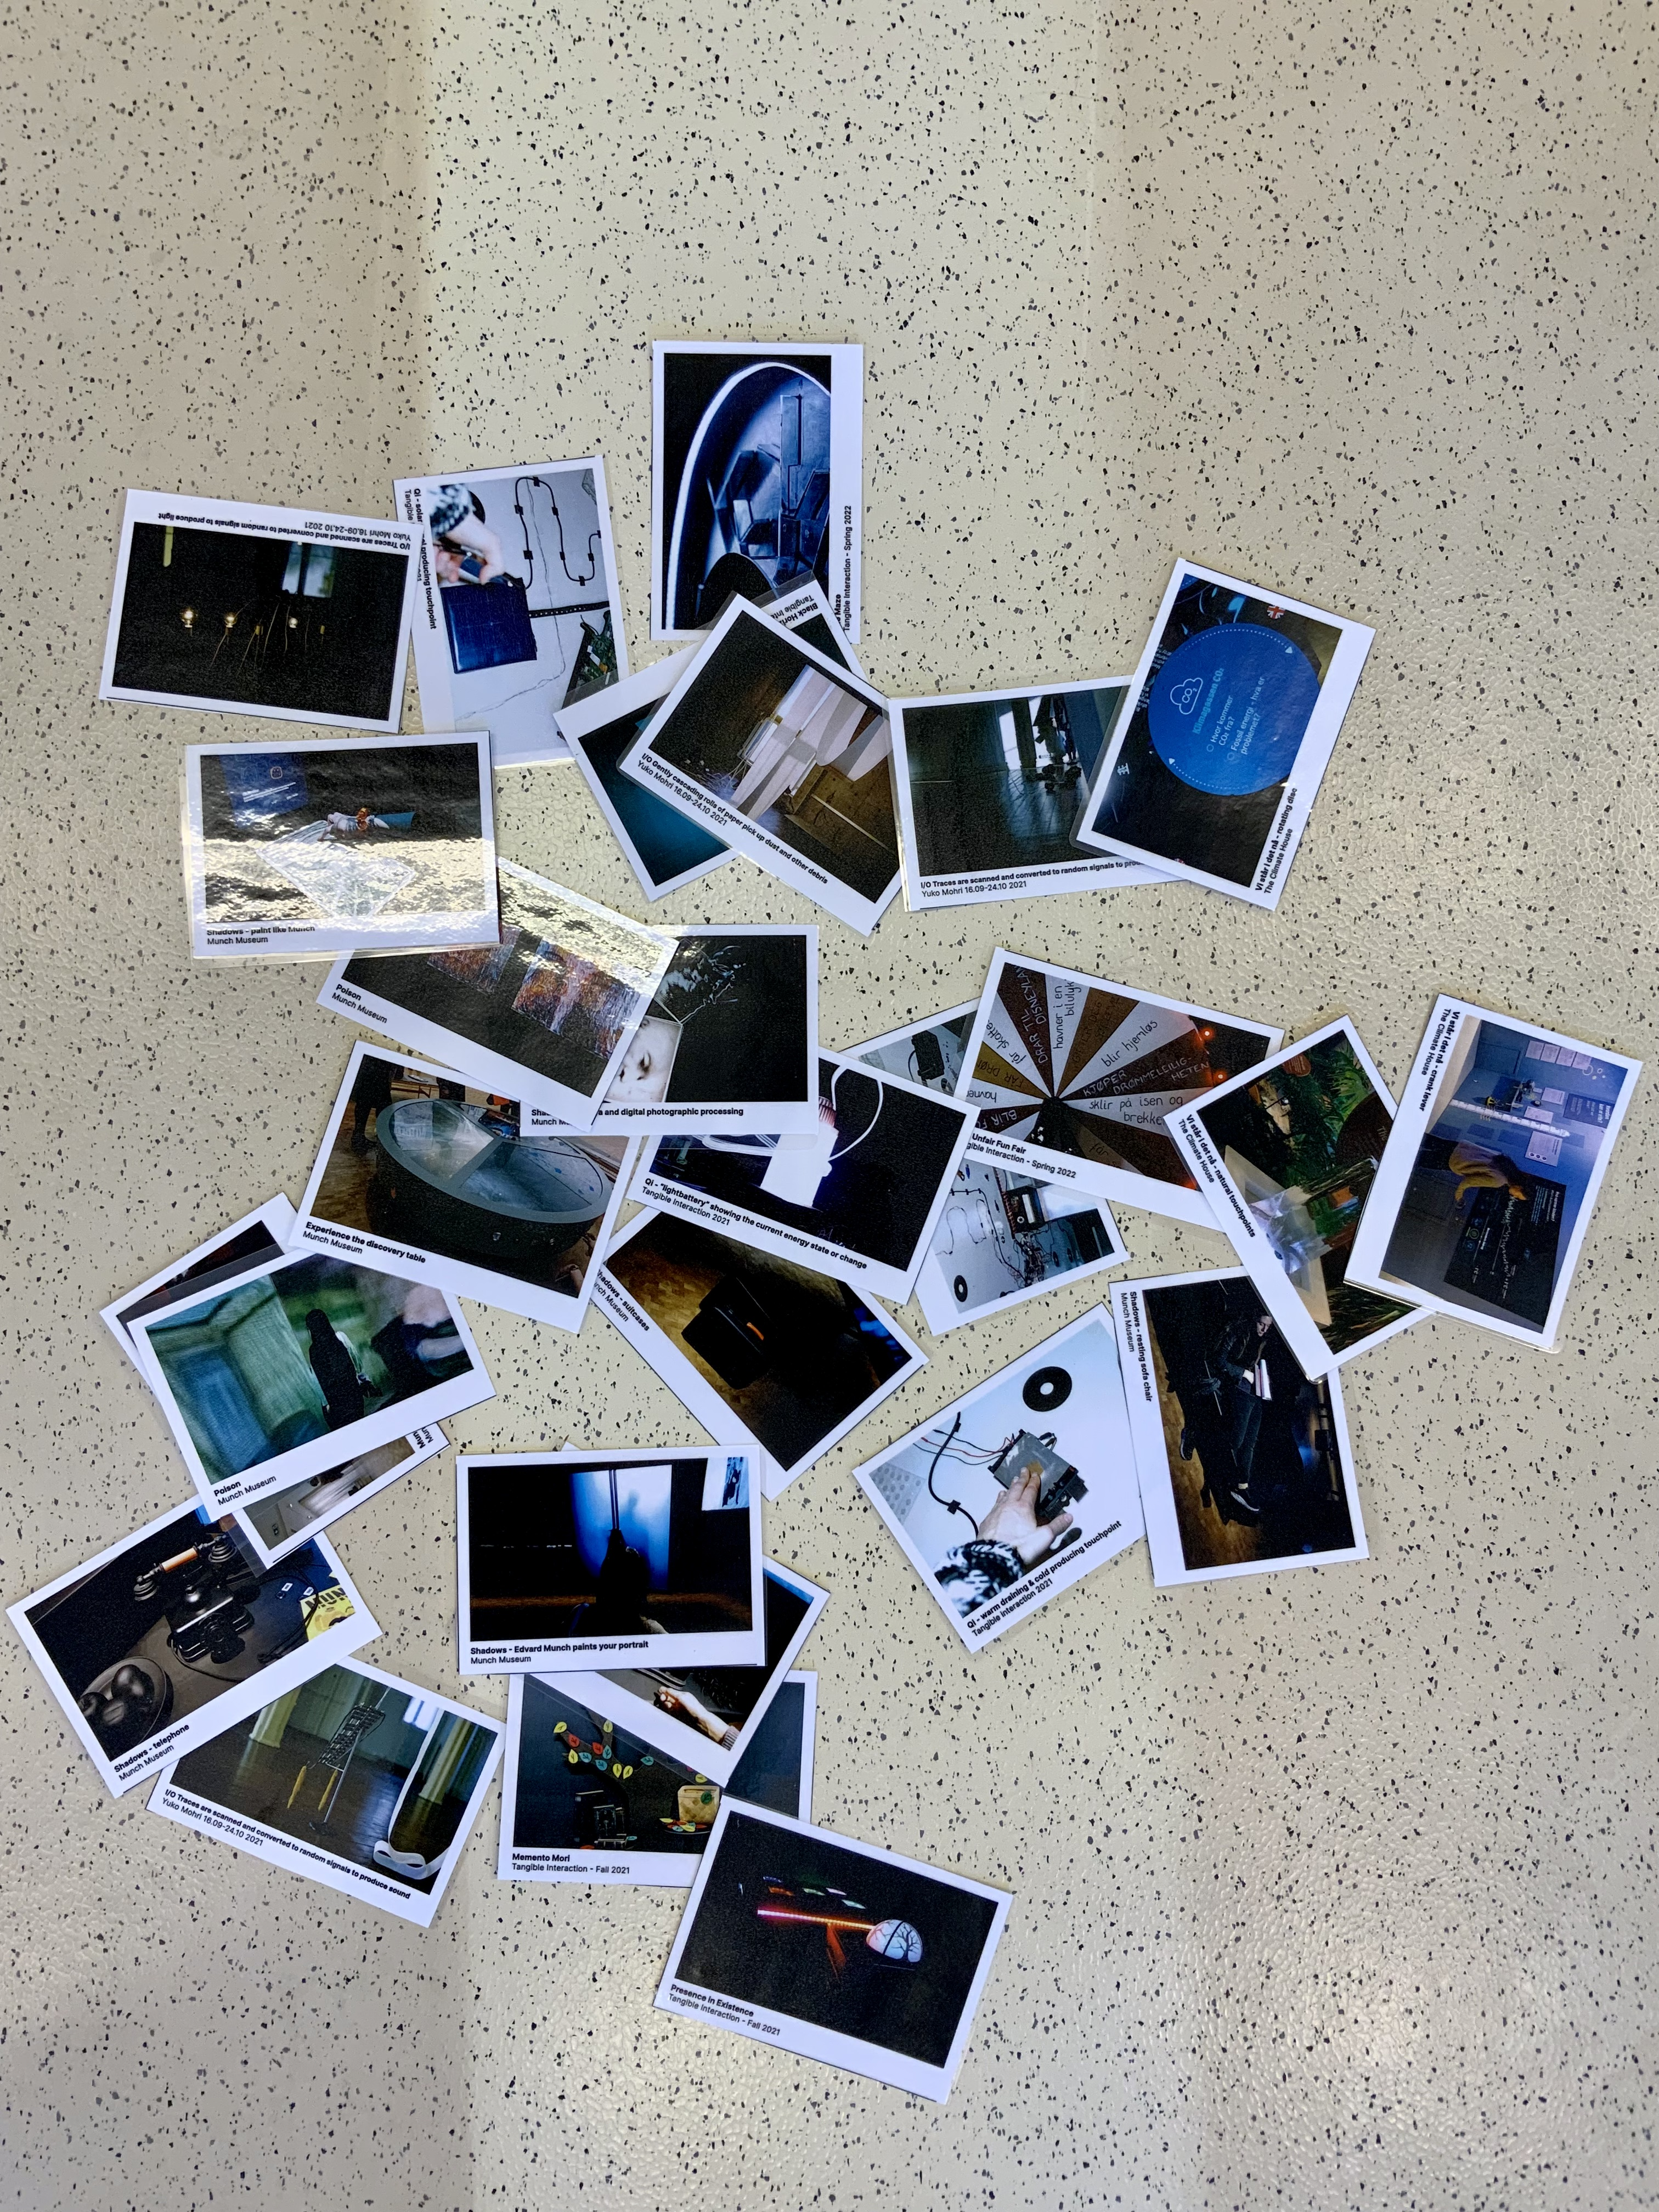
\includegraphics[width=12cm]{pictures/dataset/datasett_oversikt.jpeg}
\centering 
\end{figure}

I think this is basic qualitative analysis?

Måten jeg har gått frem på ved bruk av dette datasettet, sett opp mot mine utvalgte teorier, har vært en form for deduktiv systematisk prosess. Det vil si at jeg til å begynne med har systematisert og kategorisert installasjonene opp mot hver teori; feks som jeg har gjort her fra en av de interaktive installasjonene på klimahuset haar jeg

\subsection{"data laundering"}
Write out:
\begin{itemize}
    \item explain why munch shadows is analysed as one. and only weighted as one. and how that affects the dataset.
    \item discuss how the amount of tangible installations affect the dataset
    \item discuss the analog-tangible vs interactive-tangible installations (ice cube, munch peepholes and discovery table)
\end{itemize}

\begin{figure}[H]
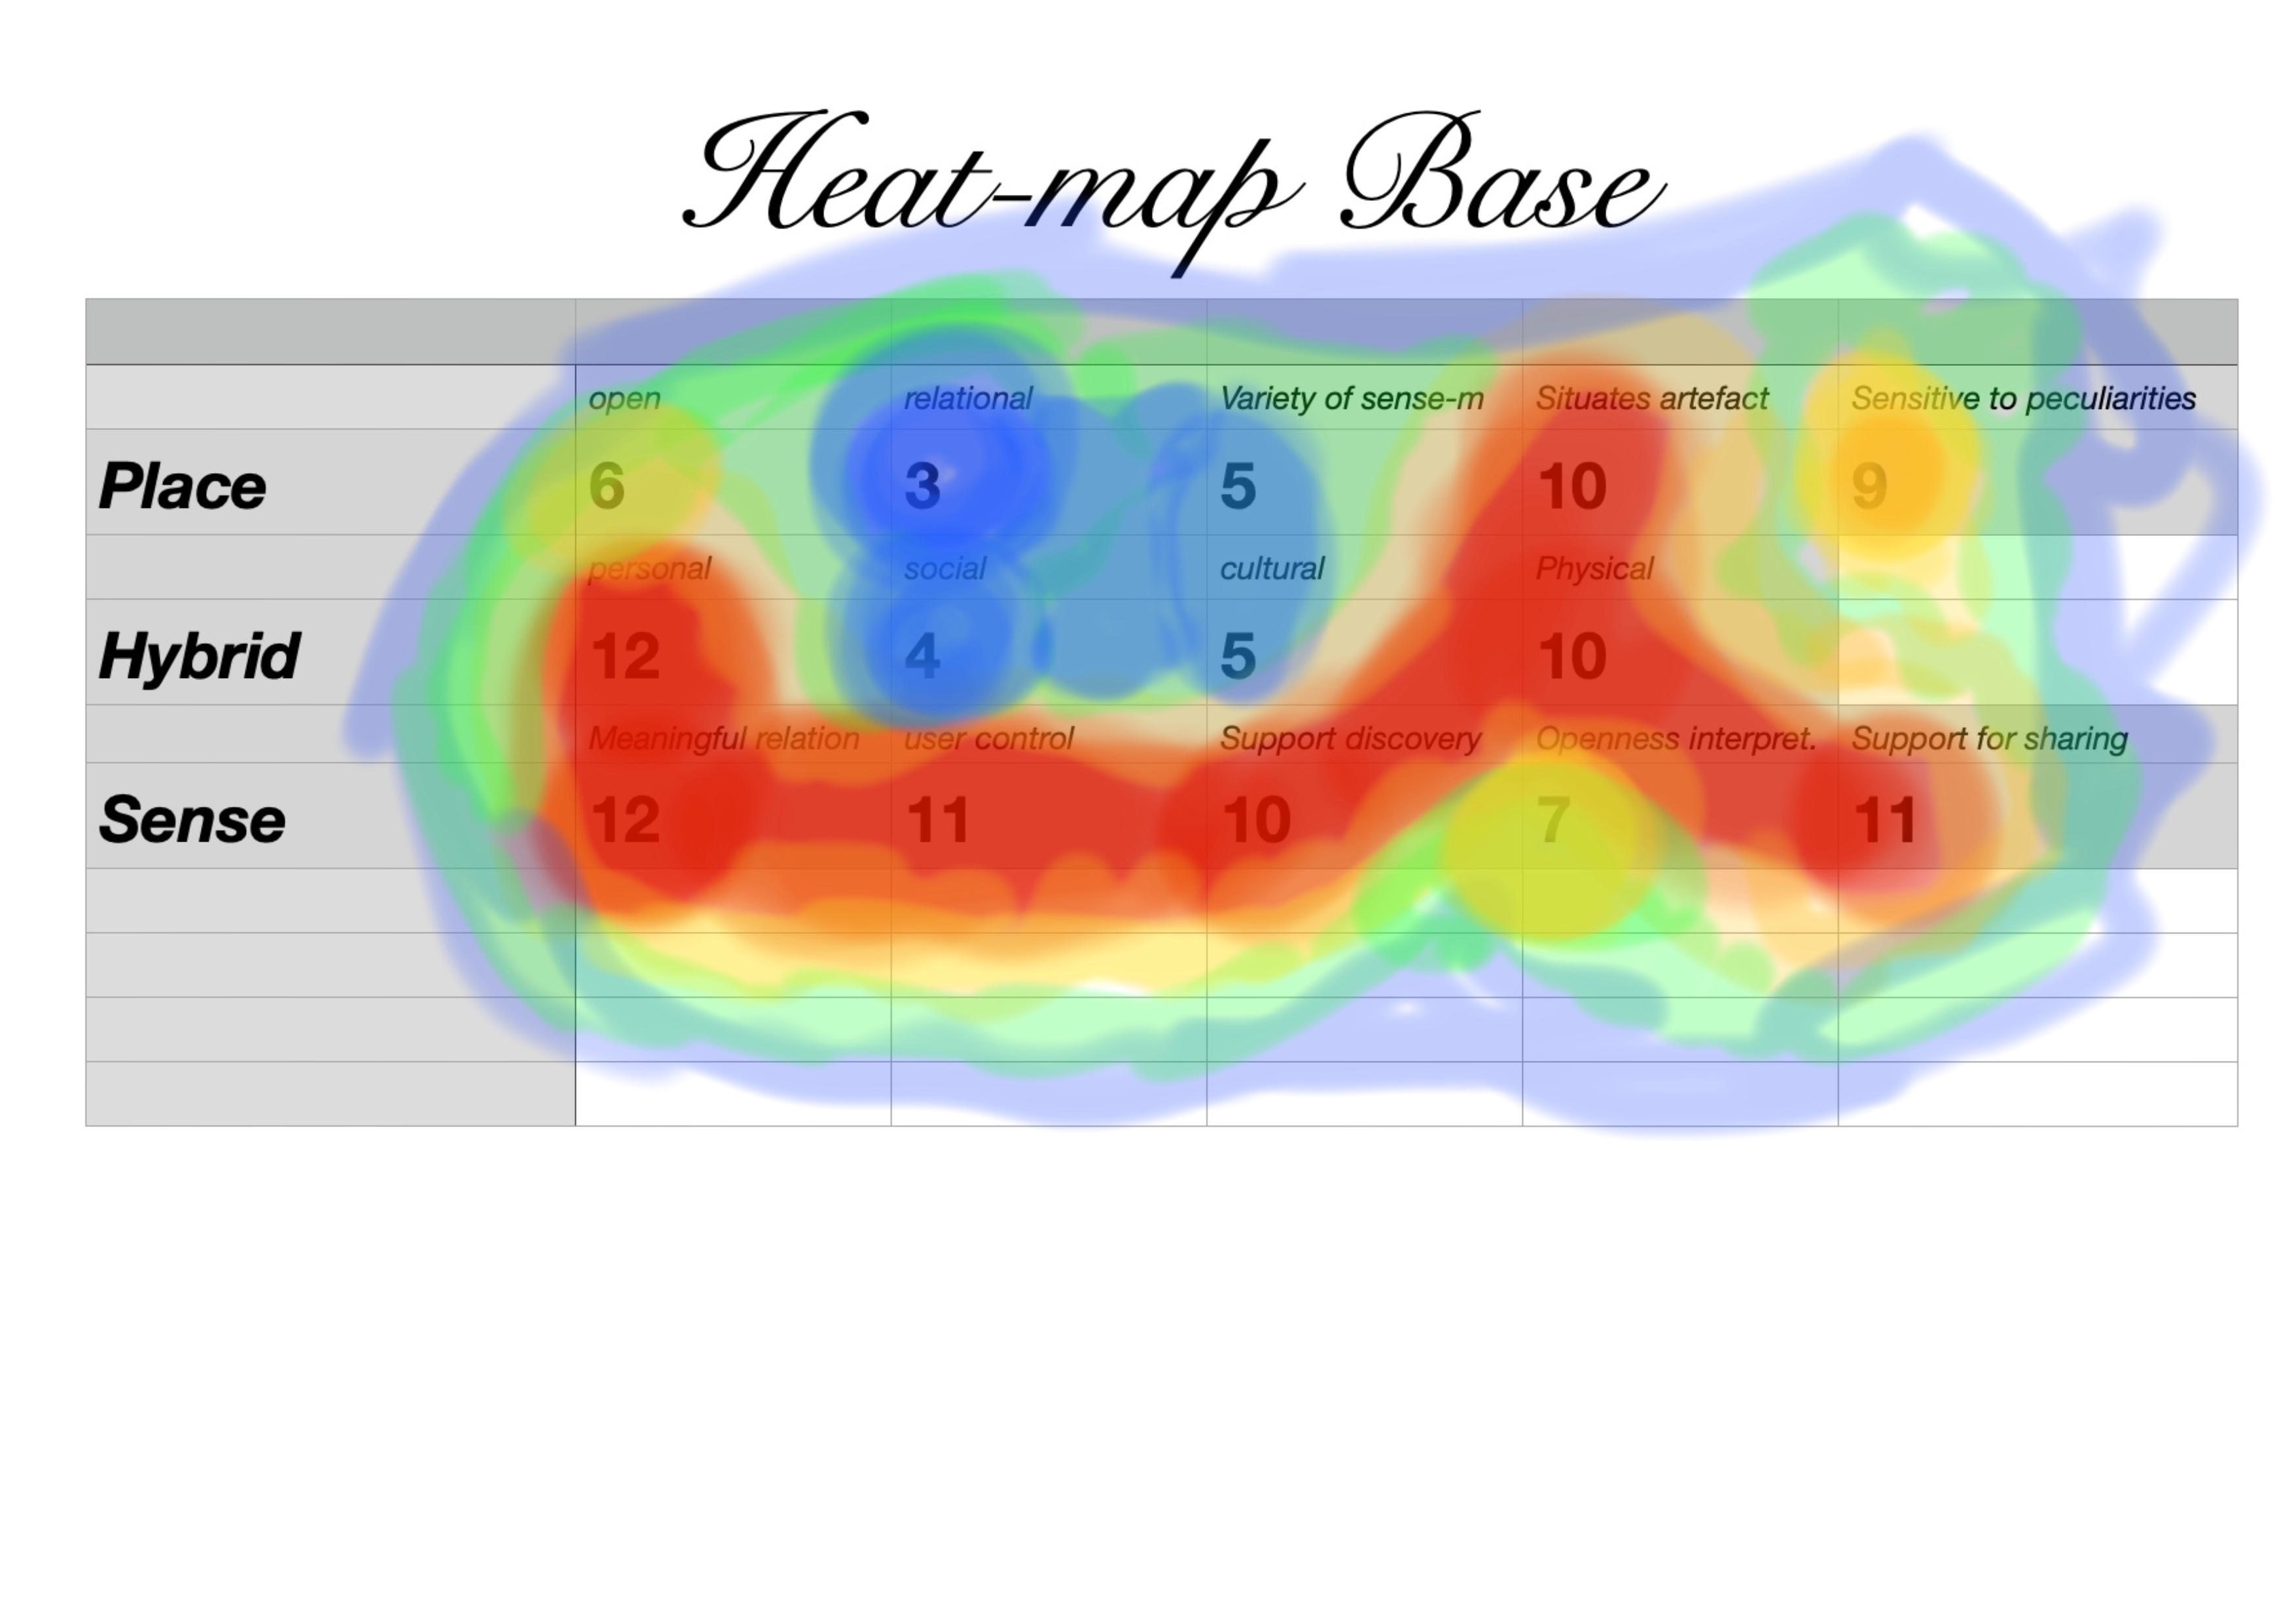
\includegraphics[width=11cm]{pictures/dataset/heatmap.jpg}
\centering 
\end{figure}


\section{First iteration: seeing the bigger picture}

I started the first analytical iteration by sorting the dataset into the three theories I base my understanding of meaningfulness on; \emph{Hybrid place, place as a dialogue} and \emph{Sense-making strategies}. I made one table for each theory, where the frameworks's principles/ and dimensions formed the columns and the 22 different installations the rows. I then went through each installation and plotted in whether or not the installation fulfilled the principle/ dimension. Categorising it this way opened up for looking at the dataset in correlation with each theory separately, making it possible to see overall trends in the dataset according to the theories. Another


respective theory from a birds-eye, holistic, perspective, but it will also work as a quick-reference guide for the second analysis iteration when I'm trying to merge the three theories and/ or finding new relationships between the data across the theories.

The categorisation of the data is highly subjective, but theoretically grounded, based on my personal experience with- and interpretation of the installations and knowledge of the museum institution the installation was part of. I have also chosen to merge all the Munch - \emph{Shadows} installations as one, because they are a part of the same exhibition and do not differ in their interactive qualities. Because of this, the dataset used for this analysis shrinked from 22 to 16. This choice of merging the \emph{Shadows} installations was made in the process of fitting the installations into the theory's principles/ dimensions, when I saw that they all checked the same boxes. 


\begin{figure}[H]
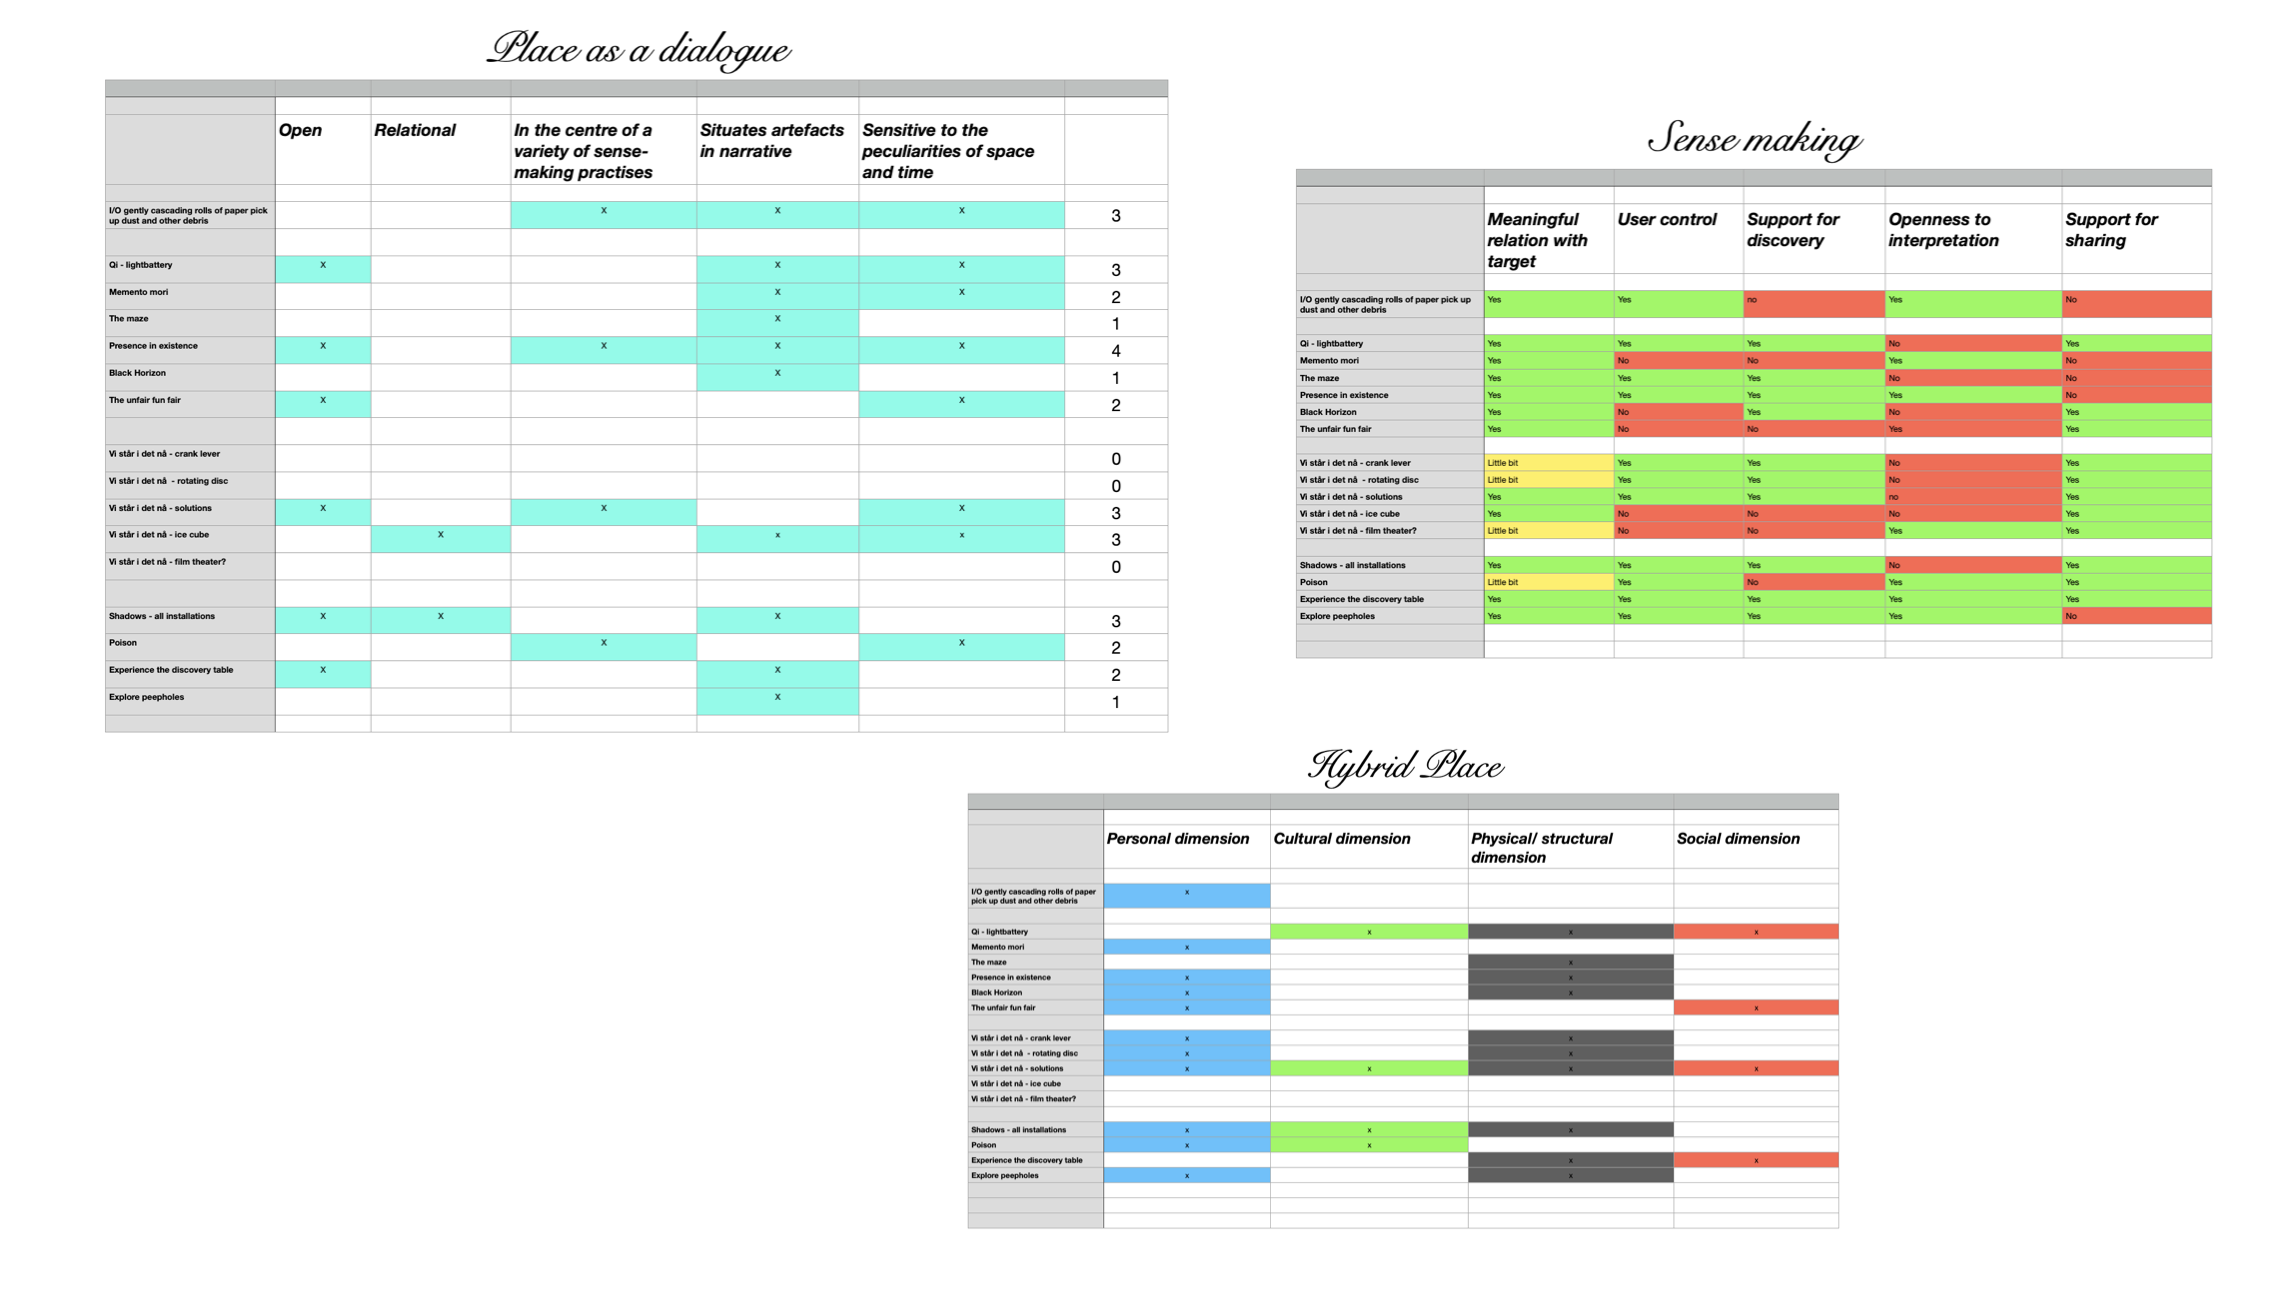
\includegraphics[width=13cm]{pictures/dataset/analysis_tables.png}
\centering 
\end{figure}

After mapping the installations in the tables, it opened up for crunching the first numbers. In this iteration I want to see the dataset from a holistic view. Abstracting from the details and seeing how the installations map up in the bigger picture. To do this I needed a diagram that could compare the different principles up against eachother. I chose to create radar charts to do this, and made a radar chart for each theory. 

\begin{figure}[H]
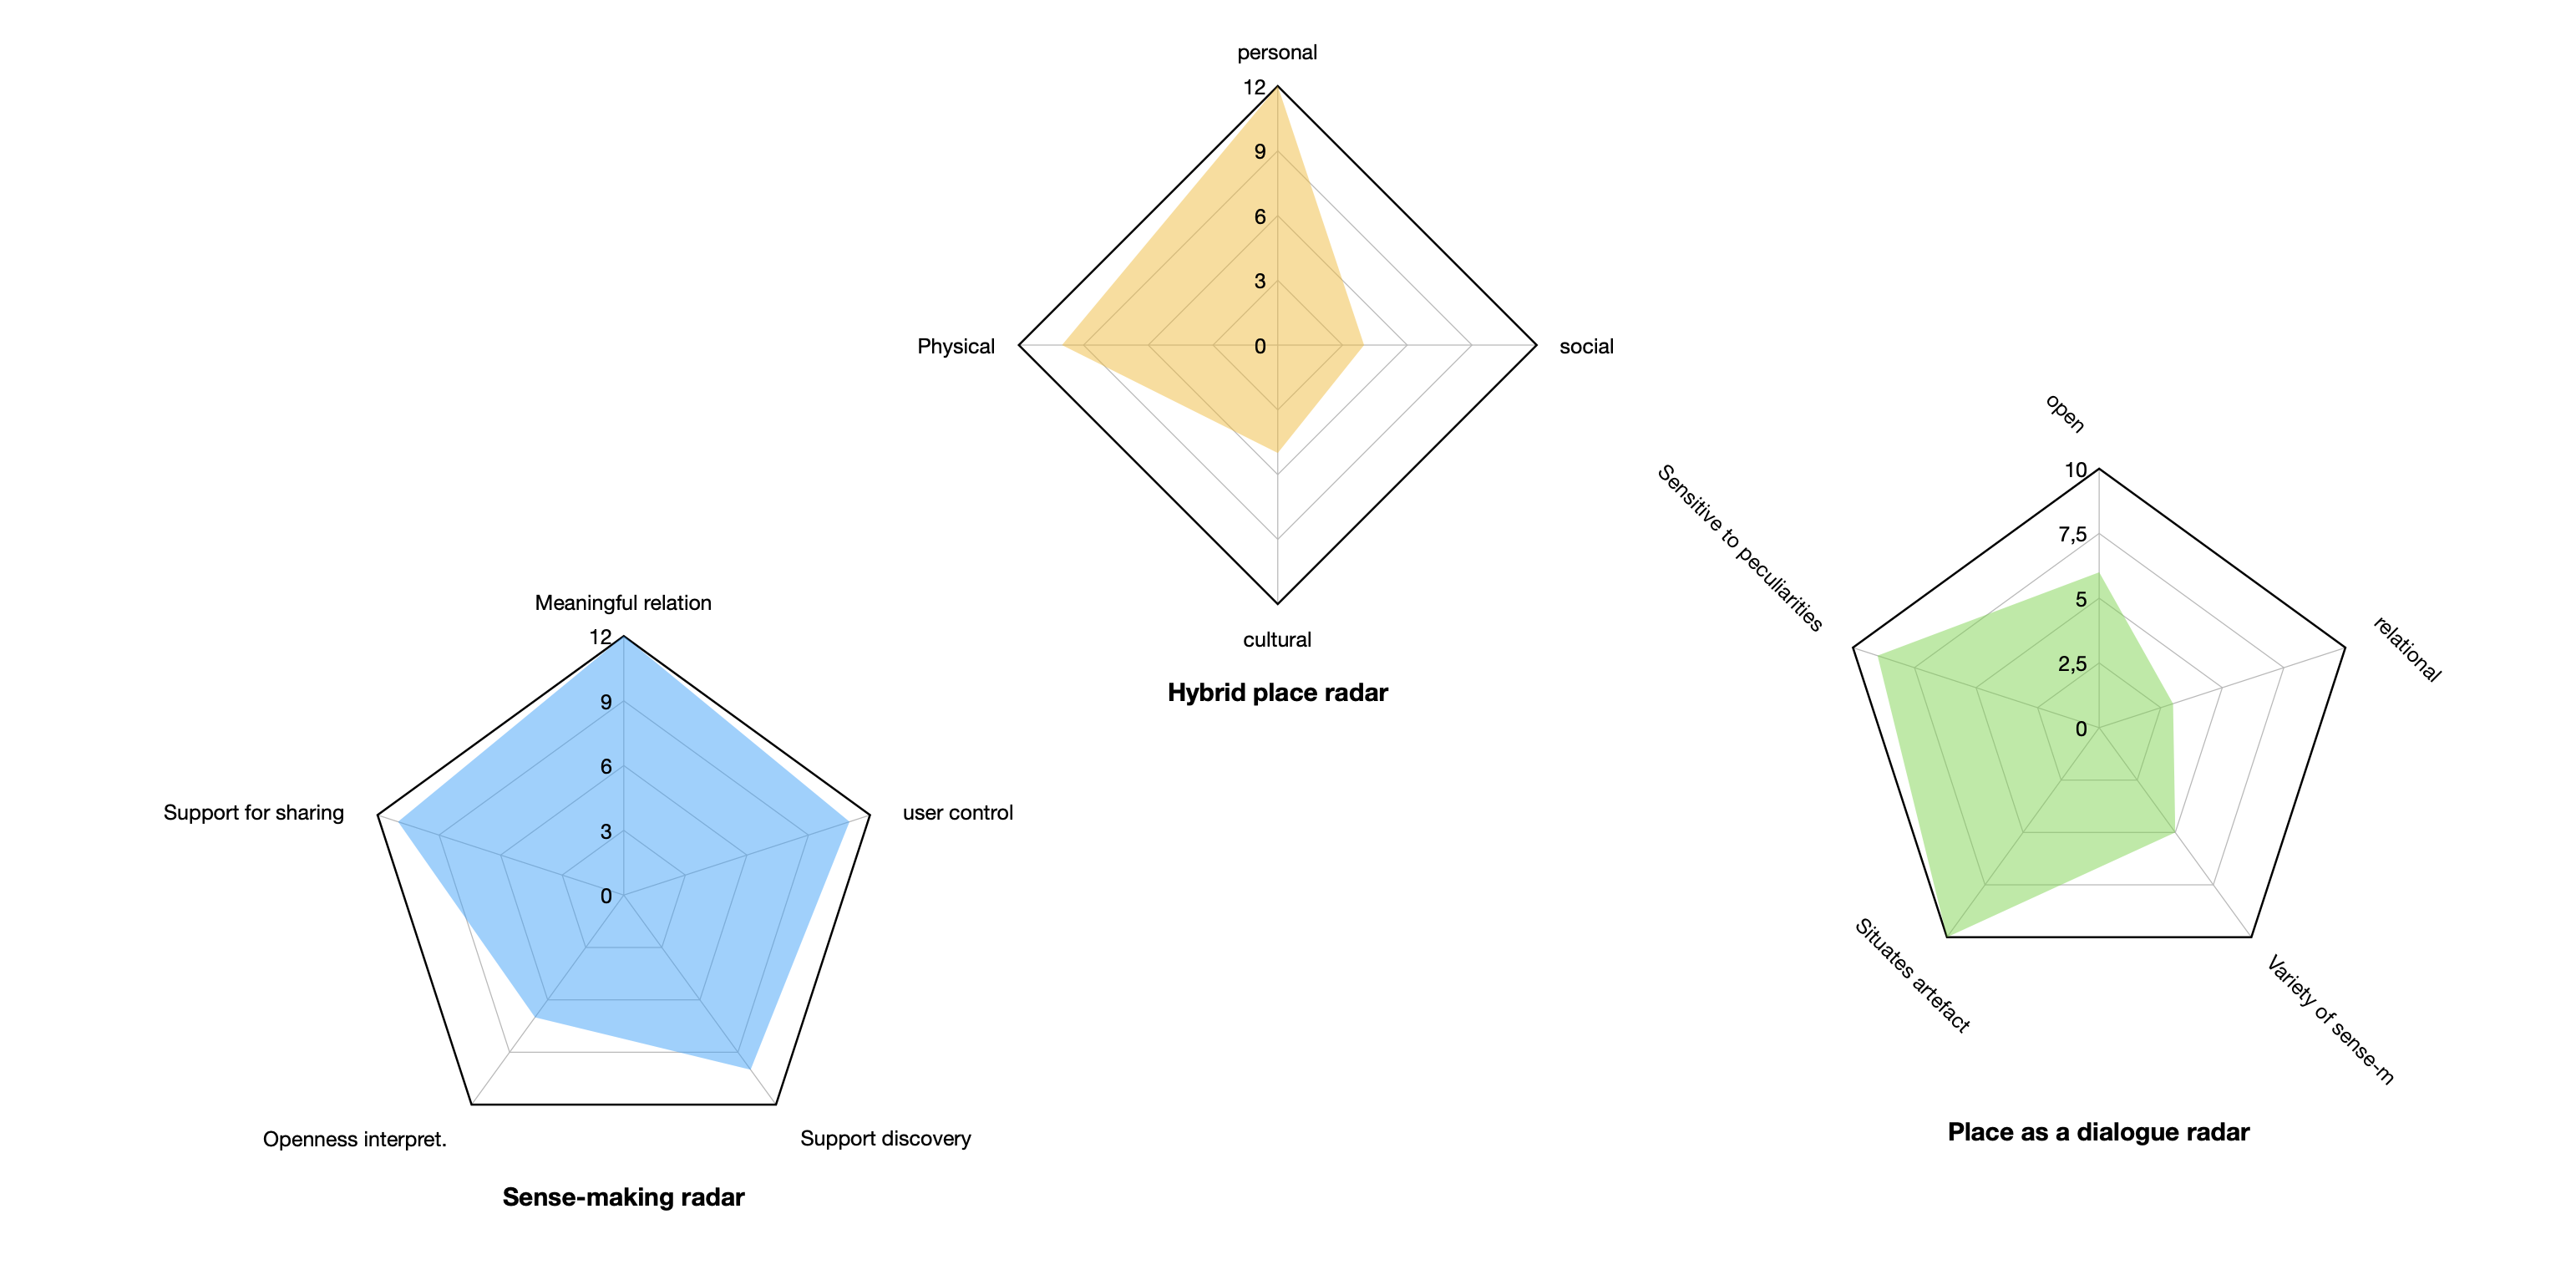
\includegraphics[width=13cm]{pictures/dataset/analysis_radars.png}
\centering 
\end{figure}

\emph{"Findings"}
\par

What I have learned by looking at the radar charts so far is how the different theories fulfill, or complement eachother. The way I have gone forward in looking at the radar charts is as following:
\par I'll start by looking at the hybrid place radar chart, noticing how the personal and physical dimension is fulfilled, while the social and cultural dimension is very little fulfilled. What does this mean? According to the Norwegian museum policy strategic thinking, it is wanted that museums transition from the personal dimension to the more social and cultural dimension. The fact that installations in my analysis shows presence in the physical dimension is positive, in terms of enabling the personal dimension, experience-wise, to involve more tangible or at least dynamic experiences in the museum space.
\par Then, if we shift focus for a second to look into the sense-making radar chart, we see that one of the corners that is fulfilled by almost all installations in this analysis - support for sharing is fulfilled. How come, that even though the social dimension is not fulfilled while almost all installations, in terms of sense-making have good support for sharing? 

\par Then again, we can look at what dialogic qualities the installations turns out to have little "relationalness", which is a dialogic principle/ quality that involves the Docents in the museum for example, or relational qualitites.


